\documentclass[12pt]{article}
\usepackage{amsmath, amssymb}
\usepackage{graphicx}
\usepackage{tikz}
\usepackage[margin=1in]{geometry}
\usepackage{float} % For the H specifier

\title{Ejercicios de grafos}
\date{29 de Agosto de 2023}

\begin{document}

\maketitle

\section*{Problema 4}
Considera \( G \) una gráfica de orden \( n = 8 \) y tamaño \( m = 15 \) en la cual cada vértice es de grado 3 o 5. ¿Cuántos vértices de grado cinco tiene \( G \)?
\begin{enumerate}
	\item Supongamos que la gráfica \( G \) tiene \( x \) vértices de grado 5 y \( y \) vértices de grado 3.
	\item Dado que la gráfica tiene un total de \( n = 8 \) vértices, podemos establecer:
	      \[ x + y = 8 \]
	      (es decir, la suma de vértices de grado 5 y vértices de grado 3 es 8).
	\item Cada vértice de grado 5 contribuye con 5 aristas y cada vértice de grado 3 contribuye con 3 aristas. Pero, cada arista se cuenta dos veces (una vez por cada vértice que incide en ella). Por lo tanto, el total de aristas \( m \) es:
	      \[ \frac{5x + 3y}{2} = 15 \]
	      (es decir, la suma ponderada de los vértices de grado 5 y 3, dividido por 2, es igual al total de aristas).
	\item Ahora, tenemos un sistema de ecuaciones con dos incógnitas:
	      \begin{align*}
		      x + y             & = 8 \quad (i)   \\
		      \frac{5x + 3y}{2} & = 15 \quad (ii)
	      \end{align*}
	      Resolviendo este sistema, encontramos que \( x = 3 \). Es decir, la gráfica \( G \) tiene 3 vértices de grado 5.
\end{enumerate}



\section*{Problema 5}
Dada la siguiente gráfica \( G' \):

\begin{enumerate}
\begin{enumerate}
\item Encuentra una subgráfica generadora tal que todo vértice tenga grado 4.
	\begin{figure}[h]
	\centering
	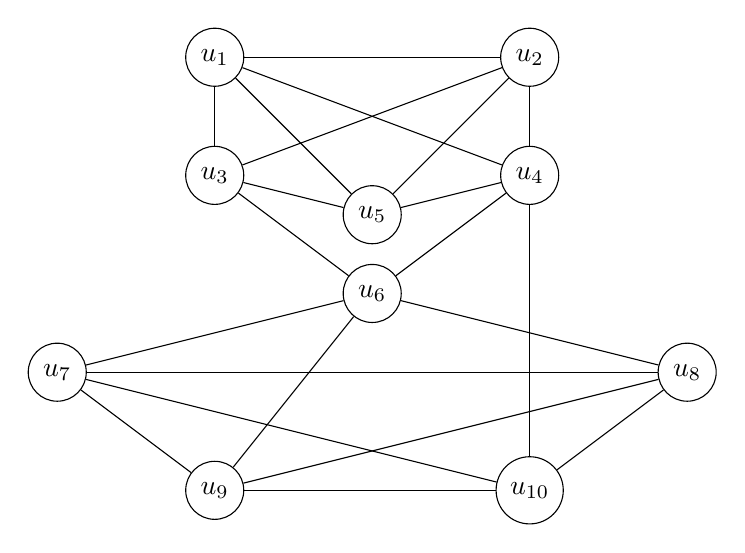
\begin{tikzpicture}
		% Vertices
		\node[draw, circle] (u1) at (0,5) {\( u_1 \)};
		\node[draw, circle] (u2) at (4,5) {\( u_2 \)};
		\node[draw, circle] (u3) at (0,3.5) {\( u_3 \)};
		\node[draw, circle] (u4) at (4,3.5) {\( u_4 \)};
		\node[draw, circle] (u5) at (2,3) {\( u_5 \)};
		\node[draw, circle] (u6) at (2,2) {\( u_6 \)};
		\node[draw, circle] (u7) at (-2,1) {\( u_7 \)};
		\node[draw, circle] (u8) at (6,1) {\( u_8 \)};
		\node[draw, circle] (u9) at (0,-0.5) {\( u_9 \)};
		\node[draw, circle] (u10) at (4,-0.5) {\( u_{10} \)};

		% Aristas
		\draw (u1) -- (u2);
		\draw (u1) -- (u3);
		\draw (u1) -- (u4);
		\draw (u1) -- (u5);
		
		\draw (u2) -- (u3);
		\draw (u2) -- (u4);
		\draw (u2) -- (u5);

		\draw (u3) -- (u5);
		\draw (u3) -- (u6);
		
		\draw (u4) -- (u5);
		\draw (u4) -- (u6);
		\draw (u4) -- (u10);

		\draw (u6) -- (u7);
		\draw (u6) -- (u8);
		\draw (u6) -- (u9);

		\draw (u7) -- (u8);
		\draw (u7) -- (u9);
		\draw (u7) -- (u10);

		\draw (u8) -- (u9);
		\draw (u8) -- (u10);

		\draw (u9) -- (u10);

	\end{tikzpicture}
	\caption{Subgráfica generadora de \( G' \)}
	\label{fig:subgraph-gprime}
\end{figure}



	\item Dibuja a la subgráfica inducida por \( A = \{u1, u2, u10, u4, u7, u8\} \).
	      \begin{figure}[H]
		      \centering
		      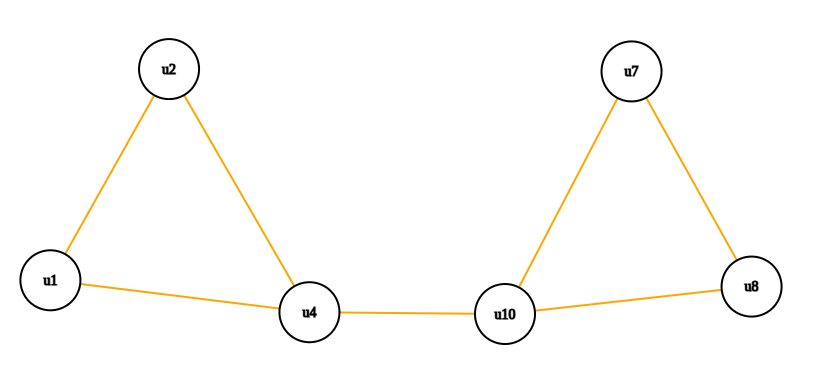
\includegraphics[width=1\textwidth]{assets/induced-subgraph.png}
		      \caption{Subgráfica inducida por \( A \)}
		      \label{fig:induced-subgraph}
	      \end{figure}

	\item Di si las gráficas \( G_1 \) y \( G_2 \) son subgráficas inducidas de \( G' \). Argumenta tus respuestas.
	      % Here, we start the representation for G'
	      \vspace{1em} % Adding vertical space for separation

	      \textbf{Respuesta:} La gráfica \( G_1 \) es una subgráfica inducida de \( G' \), ya que las conexiones entre los vértices de \( G_1 \) son las mismas que las conexiones entre los vértices de \( G' \). Por otro lado, la gráfica \( G_2 \) no es una subgráfica inducida de \( G' \), ya que los vértices \( u_6 \) y \( u_{10} \) están conectados en \( G_2 \), pero no en \( G' \).
	      \vspace{1em} % Adding vertical space for separation

	      % Representation for G'
	      \textbf{Gráfica \( G' \):}
	      \begin{center}
		      \begin{tabular}{|c|c|}
			      \hline
			      Vértices    & Aristas                                              \\
			      \hline
			      \( u_1 \)   & \( (u_1, u_2), (u_1, u_3) , (u_1, u_4),(u_1, u_5) \) \\
			      \( u_2 \)   & \( (u_2, u_3), (u_2, u_4), (u_2, u_5) \)             \\
			      \( u_3 \)   & \( (u_3, u_5), (u_3,u_6) \)                          \\
			      \( u_4 \)   & \( (u_4, u_5), (u_4,u_6),(u_4,u_{10}) \)             \\
			      \( u_5 \)   & \(  \)                                               \\
			      \( u_6 \)   & \( (u_6, u_7) , (u_6,u_8), (u_6,u_9)\)               \\
			      \(u_7 \)    & \( (u_7, u_8) , (u_7,u_9),(u_7,u_{10}) \)            \\
			      \(u_8 \)    & \( (u_8, u_9) , (u_8,u_{10}) \)                      \\
			      \(u_9 \)    & \( (u_9, u_{10}) \)                                  \\
			      \(u_{10} \) & \(  \)                                               \\
			      \hline
		      \end{tabular}
	      \end{center}

	      \vspace{1em} % Adding vertical space for separation

	      % Representation for G1
	      \textbf{Gráfica \( G_1 \):}
	      \begin{center}
		      \begin{tabular}{|c|c|}
			      \hline
			      Vértices  & Aristas                                    \\
			      \hline
			      \( u_1 \) & \( (u_1, u_2), (u_1, u_3) , (u_1, u_4), \) \\
			      \( u_2 \) & \( (u_2, u_3), (u_2, u_4) \)               \\
			      \( u_3 \) & \( (u_3, u_6) \)                           \\
			      \( u_4 \) & \( (u_4, u_6) \)                           \\
			      \( u_6 \) & \( (u_6, u_7) , (u_6,u_9) \)               \\
			      \( u_7 \) & \( (u_7, u_9) \)                           \\
			      \( u_9 \) & \( \)                                      \\
			      \hline
		      \end{tabular}
	      \end{center}

	      \vspace{1em} % Adding vertical space for separation

	      % Representation for G2
	      \textbf{Gráfica \( G_2 \):}
	      \begin{center}
		      \begin{tabular}{|c|c|}
			      \hline
			      Vértices     & Aristas                                   \\
			      \hline
			      \( u_2 \)    & \( (u_2, u_3), (u_2, u_4), (u_2,u_5) \)   \\
			      \( u_3 \)    & \( (u_3, u_5), (u_3,u_6) \)               \\
			      \( u_4 \)    & \( (u_4, u_5), (u_4,u_{10}) \)            \\
			      \( u_5 \)    & \(  \)                                    \\
			      \( u_6 \)    & \( (u_6, u_8) , (u_6,u_7), (u_6,u_{10})\) \\
			      \( u_7 \)    & \( (u_7, u_8) , (u_7,u_{10}) \)           \\
			      \( u_8 \)    & \( (u_8, u_{10}) \)                       \\
			      \( u_{10} \) & \(  \)                                    \\
			      \hline
		      \end{tabular}
	      \end{center}

\end{enumerate}


\section*{Problema 6}
Da un ejemplo de dos gráficas \( G \) y \( H \) y una función biyectiva \( f: V(G) \rightarrow V(H) \) tal que si \( uv \in E(G) \), entonces \( f(u)f(v) \in E(H) \), pero que \( G \) y \( H \) no sean isomorfas.

\subsection*{Gráfica \( G \)}
\begin{center}
	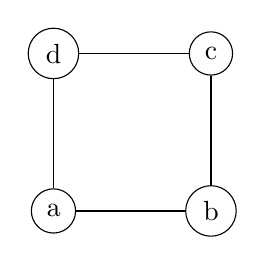
\begin{tikzpicture}
		\node[draw, circle] (a) at (0,0) {a};
		\node[draw, circle] (b) at (2,0) {b};
		\node[draw, circle] (c) at (2,2) {c};
		\node[draw, circle] (d) at (0,2) {d};

		\draw (a) -- (b) -- (c) -- (d) -- (a);
	\end{tikzpicture}
\end{center}

\subsection*{Gráfica \( H \)}
\begin{center}
	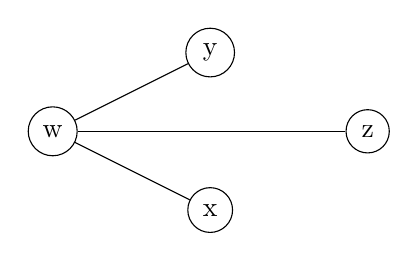
\begin{tikzpicture}
		\node[draw, circle] (w) at (4,1) {w};
		\node[draw, circle] (x) at (6,0) {x};
		\node[draw, circle] (y) at (6,2) {y};
		\node[draw, circle] (z) at (8,1) {z};

		\draw (w) -- (x);
		\draw (w) -- (y);
		\draw (w) -- (z);
	\end{tikzpicture}
\end{center}

\textbf{Justificación:}

Las gráficas \( G \) y \( H \) tienen una función biyectiva \( f \) definida de la siguiente manera:
- \( f(a) = w \)
- \( f(b) = x \)
- \( f(c) = y \)
- \( f(d) = z \)

Esta función mapea cada vértice de \( G \) a un vértice de \( H \), y si hay una arista entre dos vértices en \( G \), entonces también hay una arista entre sus imágenes en \( H \). Sin embargo, las gráficas no son isomorfas debido a sus estructuras intrínsecas.

\( G \) es un ciclo, lo que significa que puedes empezar en cualquier vértice y seguir las aristas para regresar al punto de partida sin repetir ninguna arista. Por otro lado, \( H \) es una estrella, con un vértice central conectado a todos los demás vértices, pero esos vértices exteriores no están conectados entre sí. Estas estructuras son fundamentalmente diferentes, lo que significa que no hay manera de "reorganizar" o "re-etiquetar" una gráfica para que se parezca a la otra, y por lo tanto, las gráficas no son isomorfas.




\end{document}
